\documentclass[a4paper]{article}
\usepackage[T1]{fontenc}
\usepackage[utf8]{inputenc}
\usepackage[finnish]{babel}
\usepackage[pdfborder={0 0 0}]{hyperref}
\usepackage{graphicx}
\usepackage[scale=0.65]{geometry}
\title{Tietokantasovellus-harjoitustyön dokumentaatio}
\author{Miika Hänninen}
\begin{document}

\maketitle
\tableofcontents
\pagebreak

\section{Johdanto}
Tämän tietokantasovellus-harjoitustyön aiheena on drinkkiarkisto. Drinkkiarkiston tarkoitus on olla jokaisen kotibaarimestarin apuväline jolla löytää uudenlaisia juomia kokeiltavaksi, sekä palauttaa tuttujen drinkkien reseptit mieleen. Arkistosta kuka tahansa pystyy etsimään juomia esimerkiksi nimen, juomatyypin tai ainesosien perusteella. Kirjautuneet käyttäjät voivat luoda drinkkireseptejä ehdotuksiksi, jotka eivät näy suurelle yleisölle ennen kuin ylläpitäjä on ne hyväksynyt.

Projekti toteutetaan javascriptillä käyttäen alustana nodejs:ää. Tietokantana toimii PostgreSQL. Web-frameworkina toimii express. Dokumentaatio kirjoitetaan latexilla. Sovellus ei vaadi käyttäjän selaimelta javascript-tukea, joskin sitä käytetään jonkin verran parantamaan käyttökokemusta jos tuki löytyy. Sovelluksen kehittämisen helpottamiseksi projektille on vagrant-konfiguraatio. Vagrant luo virtuaalikoneen joka vastaa mahdollisimman paljon tuotantoympäristöä ja sisältää kaiken tarpeellisen sovelluksen ajamiseen. 

Valmis ohjelmisto ajetaan herokussa. Jatkuvan integroinnin palvelu Travis kääntää uuden version ohjelmistosta aina kun githubiin pushataan uusi versio lähdekoodista, ja siirtää sen suoraan herokuun.
\pagebreak

\section{Yleiskuva järjestelmästä}
\subsection{Käyttötapauskaavio}
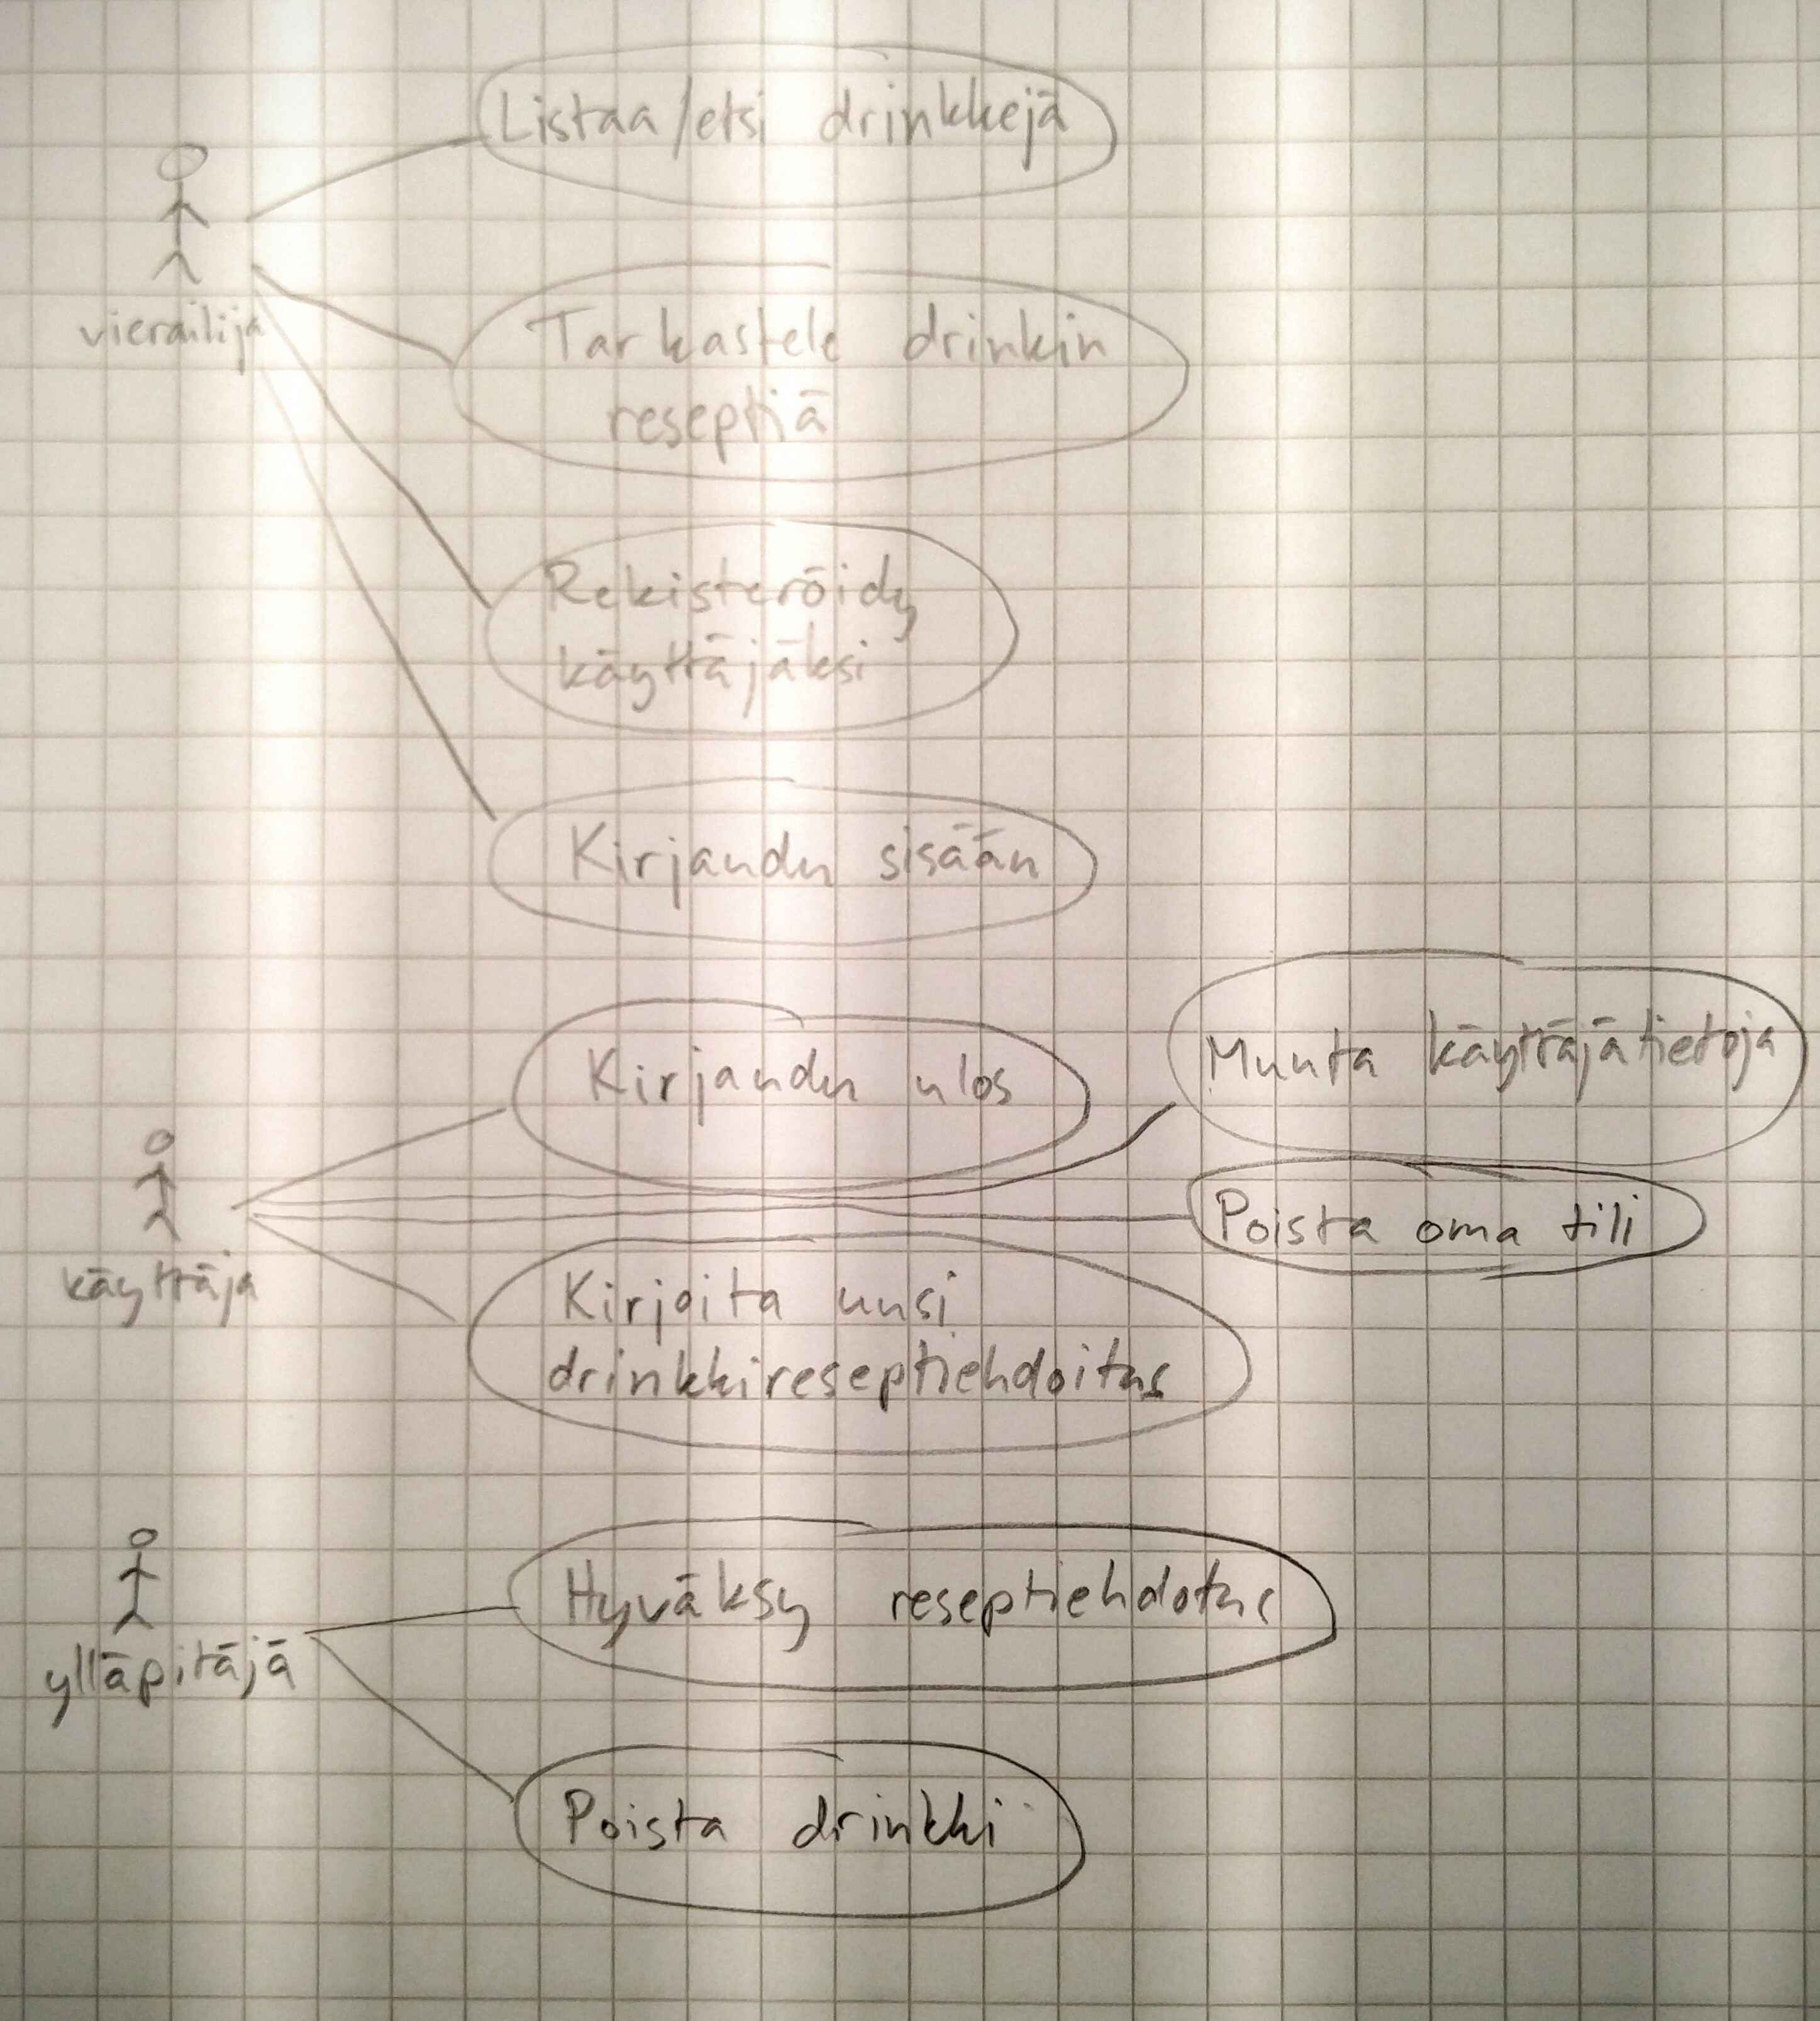
\includegraphics[width=\textwidth]{usecase-diagram}

\subsection{Käyttäjäryhmät}
\begin{description}
  \item[Vierailija] \hfill \\ Vierailijalla tarkoitetaan ketä tahansa joka vierailee sivulla.
  \item[Käyttäjä] \hfill \\ Käyttäjä on sivustolle rekisteröitynyt ja sisäänkirjautunut vierailija.
  \item[Ylläpitäjä] \hfill \\ Ylläpitäjä on käyttäjä, jonka tehtäviin ja oikeuksiin kuuluu reseptien hallinnointi.
\end{description}

\subsection{Käyttötapauskuvaukset}
\subsubsection{Vierailijan käyttötapaukset}
\begin{description}
  \item[Listaa drinkkejä] \hfill \\ Kun vierailija saapuu drinkkiarkiston etusivulle, hänelle näytetään lista uusimmista drinkeistä.
  \item[Etsi drinkkejä] \hfill \\ Drinkkiarkiston etusivulla on hakukenttä. Kun vierailija syöttää siihen hakusanan ja painaa hae-nappia (tai painaa enter), siirtyy hän hakutulossivulle joka näyttää hakua vastaavat drinkit.
  \item[Tarkastele drinkin reseptiä] \hfill \\ Kun vierailija klikkaa drinkkilistauksessa drinkin nimeä tai kuvaa, hän siirtyy reseptisivulle, jossa hän näkee drinkin tiedot tarkemmin, sisältäen drinkin ainesosat ja reseptin.
  \item[Muita käyttötapauksia] Rekisteröidy käyttäjäksi, Kirjaudu sisään
\end{description}

\subsubsection{Käyttäjän käyttötapaukset}
\begin{description}
  \item[Muuta käyttäjätietoja] \hfill \\ Kun käyttäjä on kirjautunut sisään, hänelle näytetään ''Oma profiili''-linkki. Sitä klikkaamalla käyttäjä pääsee sivulle jolla hänen tietonsa näkyvät muokattavissa tekstikentissä. Käyttäjä voi muokata tietojaan siitä, ja ''Tallenna''-nappia painamalla tallettaa muutokset.
  \item[Poista oma tili] \hfill \\ ''Oma profiili''-sivulla on nappi ''poista tili'', jota painamalla tili tuhotaan. Ennen tuhoamista sivu pyytää varmistuksen käyttäjältä.
  \item[Kirjoita uusi drinkkireseptiehdoitus] \hfill \\ Kun käyttäjä on kirjautunut sisään, hänelle näytetään ''Uusi drinkki''-linkki. Sitä klikkaamalla käyttäjä pääsee sivulle jossa on lomake uuden drinkkireseptin laatimiseen. Täytettyään lomakkeen käyttäjä painaa ''Ehdota drinkkiä''-nappia ja reseptiehdotus tallentuu tietokantaan.
  \item[Muita käyttötapauksia] Kirjaudu ulos
\end{description}
\subsubsection{Ylläpitäjän käyttötapaukset}
\begin{description}
  \item[Hyväksy reseptiehdoitus] \hfill \\ Kun ylläpitäjä on kirjautunut sisään, hänelle näytetään ''Reseptiehdotukset''-linkki. Sitä klikkaamalla ylläpitäjä pääsee sivulle joka listaa avoimet reseptiehdotukset. Hän näkee jokaisesta ehdotuksesta tarkat tiedot samalla sivulla. Jokaisen kohdalla on ''Hyväksy''- ja ''Hylkää''-napit, jotka tekevät vastaavat toimenpiteet reseptiehdotukselle.
  \item[Poista drinkki] \hfill \\ Kun ylläpitäjä tarkastelee drinkin reseptiä, hänelle näytetään ''Poista drinkki''-nappi. Sitä painamalla drinkki poistuu järjestelmästä.
\end{description}

\section{Järjestelmän tietosisältö}
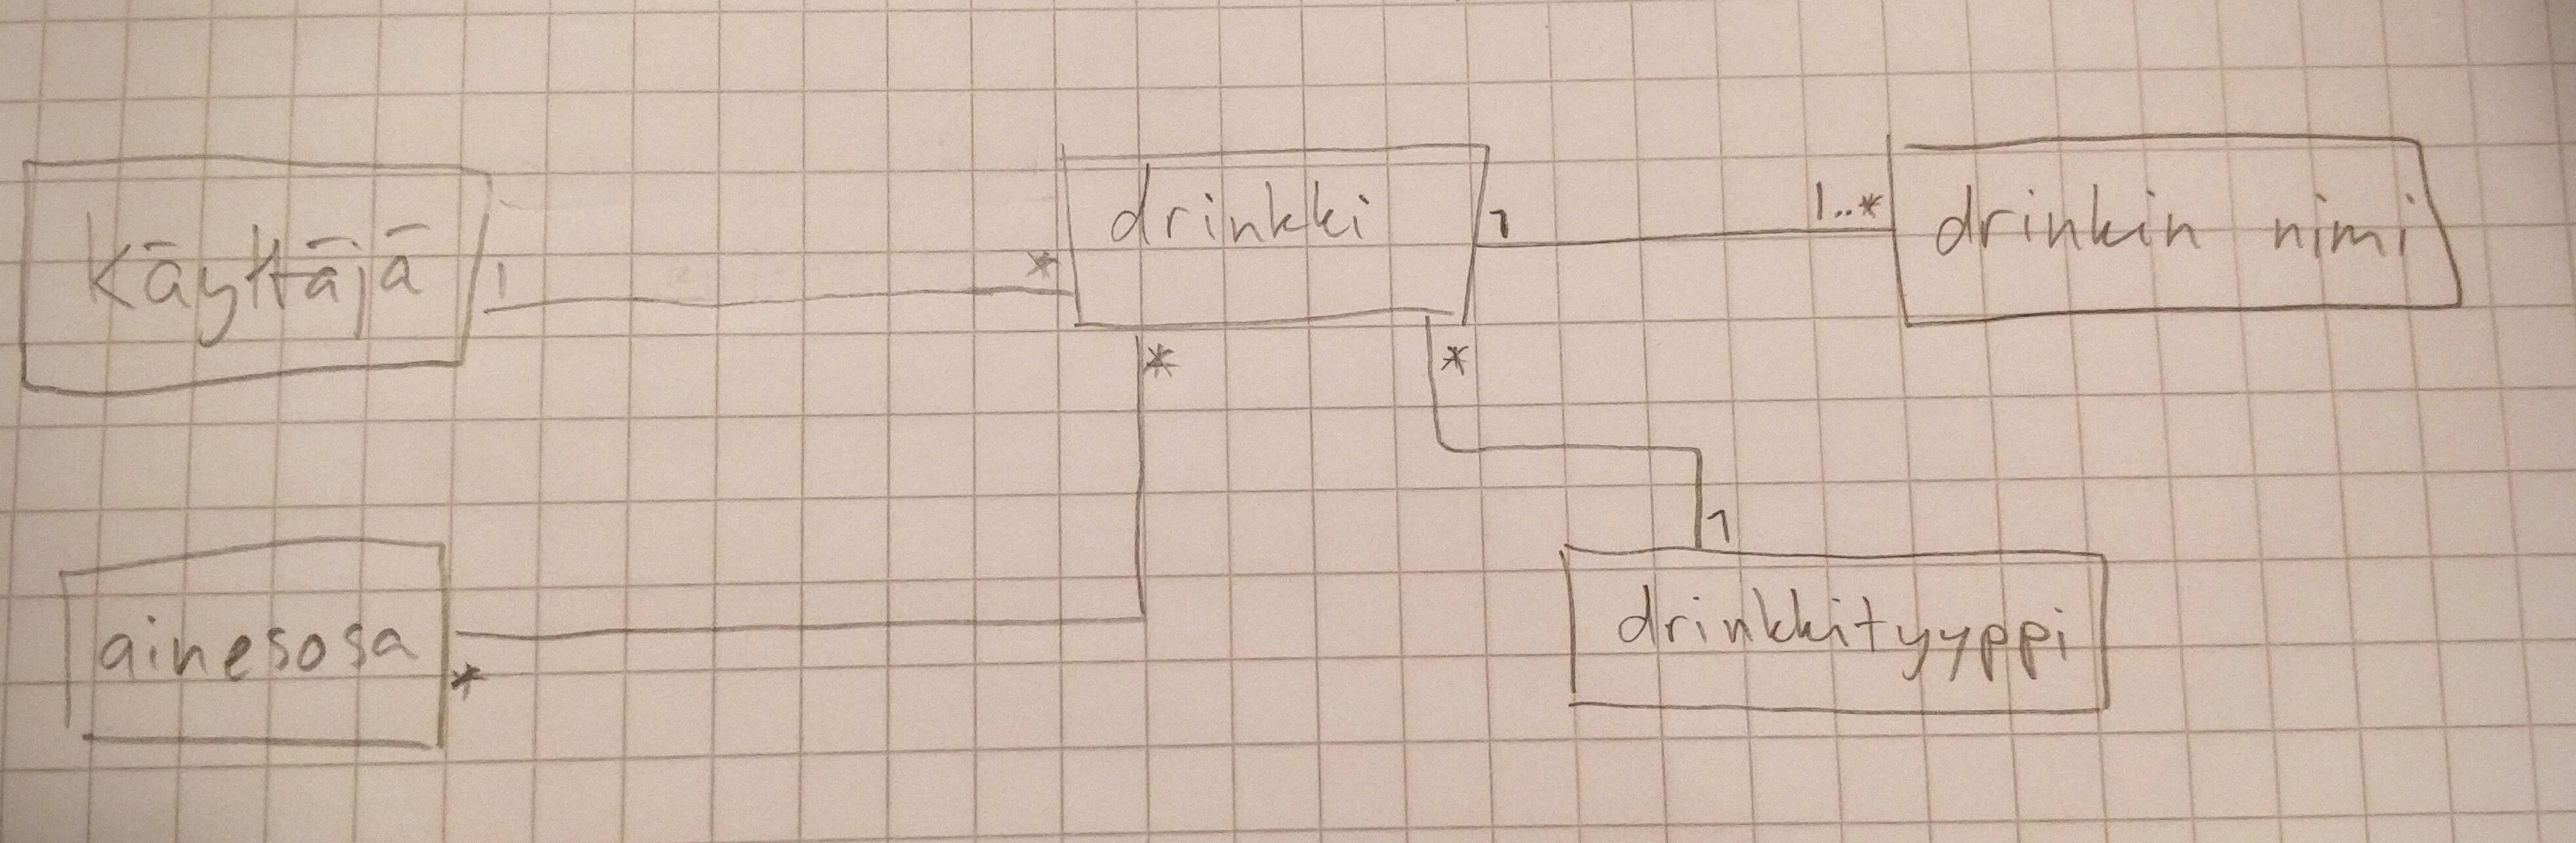
\includegraphics[width=\textwidth]{tietosisalto}

\section{Relaatiomalli}
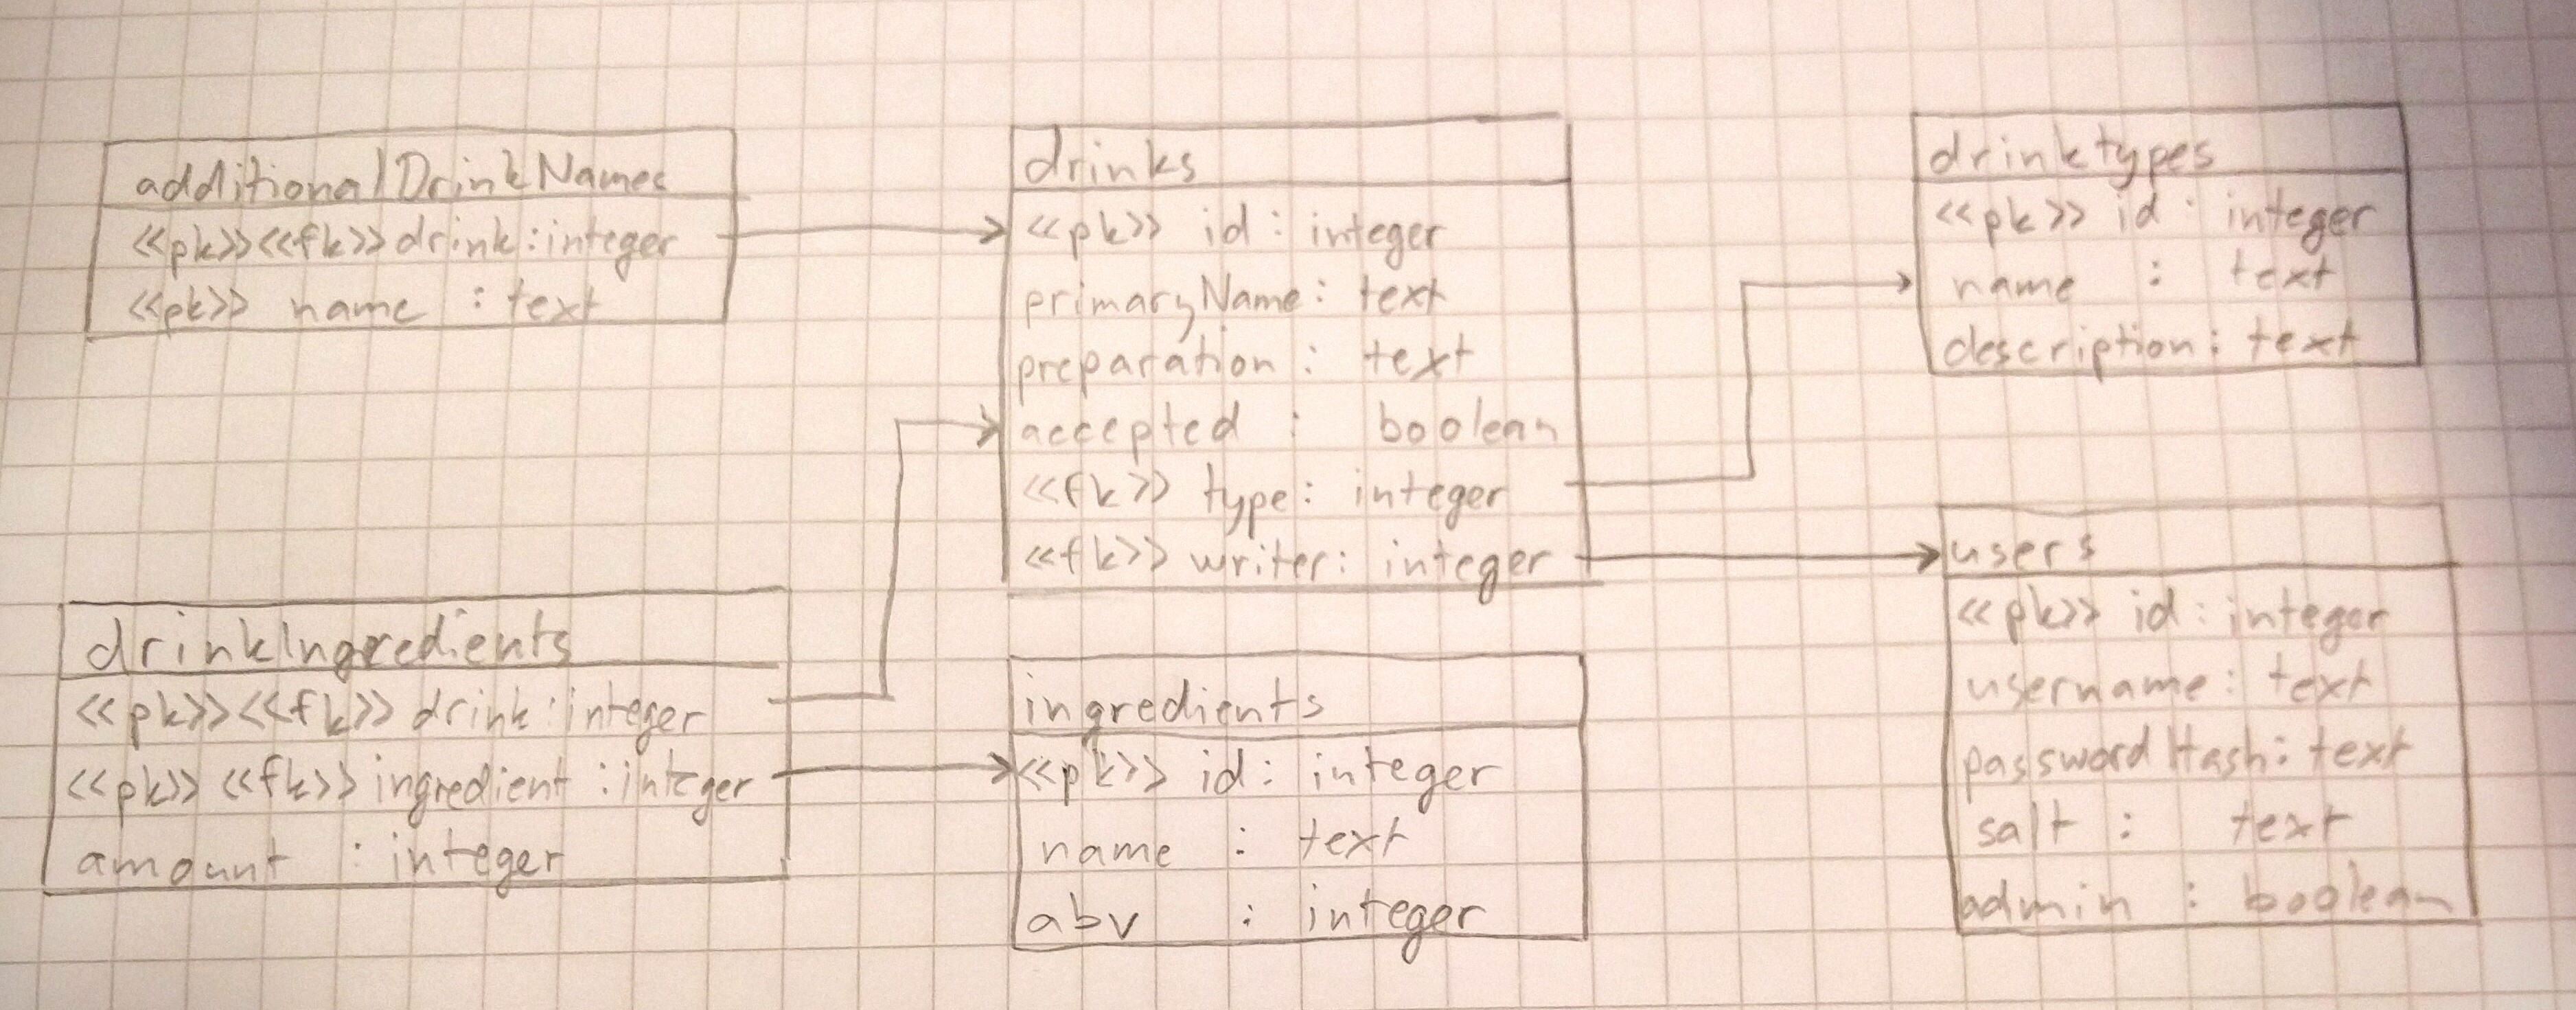
\includegraphics[width=\textwidth]{relation-diagram}

\section{Järjestelmän yleisrakenne}
\subsection{Lähdetiedostojen kansiorakenne}
\begin{description}
  \item[.editorconfig] Tekstieditorien asetuksia tälle projektille. Katso: \url{http://editorconfig.org/}
  \item[.travis.yml] Travis CI -konfiguraatio automaattisille buildeille. Katso: \url{https://travis-ci.org/}
  \item[Vagrantfile] Vagrant-kehitysympäristön konfiguraatio
  \item[bootstrap.js] Koodin entry-point. Initialisoi babelin joka kääntää es6-koodia vanhempaan syntaksiin.
  \item[doc/] Dokumentaation lähteet
  \item[scripts/] Apuriskriptejä kehitysympäristöön
  \item[sql/] Sql-skriptit mm. tietokannan, taulujen ja testidatan luontiin, sekä niiden poistamiseen
  \item[src/] Lähdekoodi ohjelmistolle.
  \item[src/controllers.js] Serverin controllerien moduuli. Kokoaa src/controllers-kansiossa olevat luokat yhteen.
  \item[src/controllers/] Serverin controlleriluokat erillisissä tiedostoissa.
  \item[src/data.js] Tietokantayhteyksien moduuli. Kokoaa src/data-kansiossa olevat luokat yhteen.
  \item[src/data/] Tietokantayhteyksien luokat yksittäisissä tiedostoissa.
  \item[src/middleware.js] Serverin middelewaret. Julkaisee serverin reiteille omia middlewareja, sekä funktion joka lisää serverin yleiset middlewaret serverille.
  \item[src/routes.js] Serverin reititystiedot.
  \item[src/server.js] Serverin päätiedosto. Konfiguroi serverin ja käynnistää sen.
  \item[src/validation.js] Serveripään datavalidoinnin moduuli. Kokoaa src/validation-kansiossa olevat luokat ja funktiot yhteen.
  \item[src/validation/] Luokkia ja funktioita datan validoimiseen serverissä.
  \item[src/views/] Näkymät ejs-templateina
  \item[vagrant/] Konfiguraatiotiedostoja kehitysympäristöön
\end{description}

\subsection{Muuta järjestelmästä}
Ohjelmisto luo session sisään kirjauduttaessa. Sessio tallennetaan sessiokeksillä joka tuhoutuu uloskirjauduttaessa tai selaimen sulkeutuessa.

Javascriptiä ei selaimen päässä käytetä tässä vaiheessa ollenkaan.

\section{Käyttöliittymä ja järjestelmän komponentit}
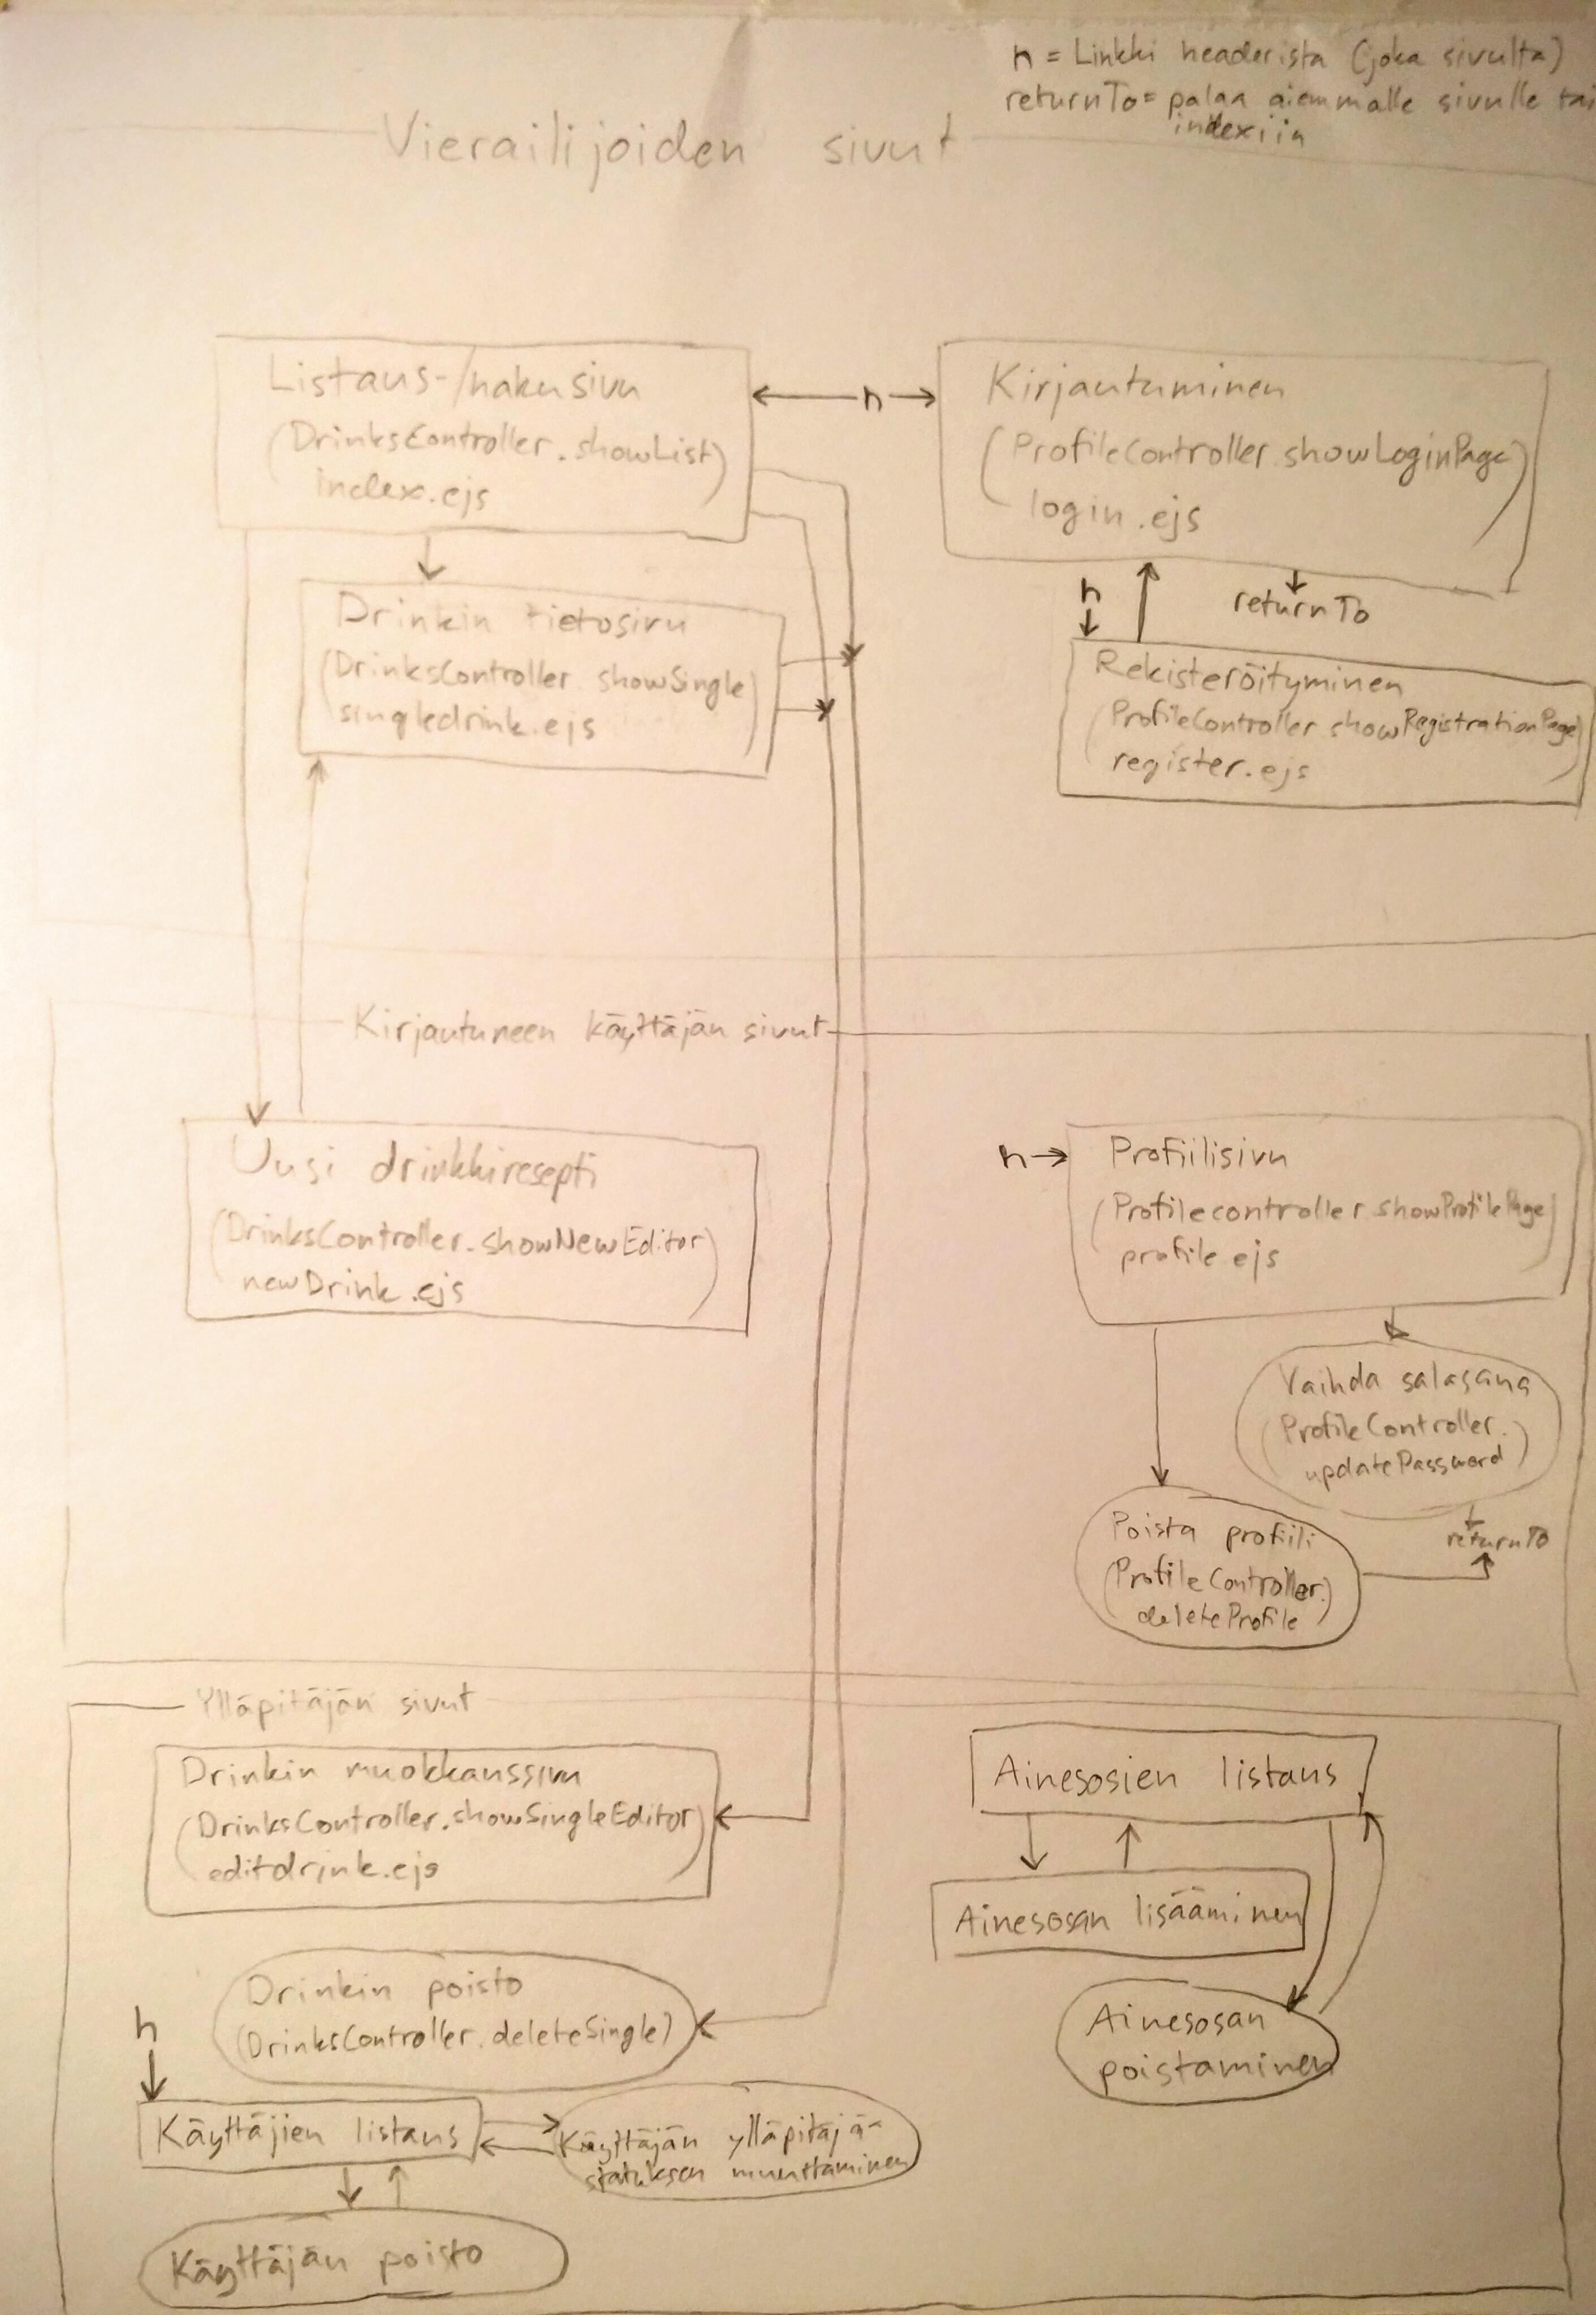
\includegraphics[width=\textwidth, height=15cm, keepaspectratio]{komponenttikaavio}

\section{Asennustiedot}
Sovellus on yksinkertaisinta asentaa Herokuun. Tällöin ei tarvita mitään ylimääräistä konfiguraatiota. Luo Herokuun uusi app, lisää siihen posgres-lisäosa, ja deployaa git pushilla ohjelmisto siihen. Tämän jälkeen aja komento \texttt{heroku run -- npm run sql \\ sql/create-tables.sql} joka lisää Herokun tietokantaan tarvittavat taulut, ja jos haluat testidatan aja \texttt{heroku run -- npm run sql sql/add-test-data.sql}.

Muualle asentaessa on asennettava node 5.x ja ympäristömuuttujaan \texttt{DATABASE\_URL} asetettava postgresin yhdistysosoite, ja ympäristömuuttujaan \texttt{PORT} tcp-portin numero jota sovelluksen halutaan kuuntelevan. Kopioi sovelluksen tiedostot johonkin sopivaan kansioon, aja sen sisällä komento \texttt{npm install} joka asentaa ohjelmiston riippuvuudet. Tämän jälkeen voit lisätä tietokantaan tarvittavat taulut komennolla \texttt{npm run sql \\ sql/create-tables.sql} ja jos haluat voit lisätä testidatan tietokantaan komennolla \texttt{npm run sql sql/add-test-data.sql}. Komento \texttt{npm start} käynnistää serverin jonka jälkeen se on tavoitettaissa ympäristömuuttujassa määritellyn portin kautta.

\section{Käynnistys- ja käyttöohje}
Ohjelmiston demoinstanssi on osoitteessa \\ \url{https://peaceful-scrubland-8625.herokuapp.com/}.

Sisään voi kirjautua yläpalkissa olevalla ''Kirjaudu sisään''-painikkeella. Käyttäjiä on kaksi: normaali käyttäjä user@example.com ja ylläpitäjä admin@example.com. Kummankin salasana on password.

Drinkkilistauksessa ja drinkkien sivuilla drinkin nimen vieressä on kuvakkeita. Kynäkuvake avaa muokkaussivun ja ruksi poistaa drinkin.

Kirjautuneet käyttäjät voivat lisätä drinkkejä, ja ylläpitäjät myös muokata ja poistaa niitä. Nappeja lisäystä, muokkausta ja poistoa varten ei näytetä, jos käyttäjällä ei ole oikeutta niihin.

\section{Testaus, tunnetut bugit ja jatkokehitys}
Testaus on tähän mennessä rajoittunut käyttäjätestaukseen. Tämä ei tietenkään ole kovin ideaalia, joten jatkossa olisikin tarkoitus lisätä ainakin automatisoituja integraatiotestauksia.

Jatkokehitysajatuksena minulla on luoda clientside-javascriptillä sujuvamman tuntuinen käyttöliittymä, käyttäen cycle.js-kirjastoa. Tämän toteutuksen pitäisi kuitenkin toimia niin, että kaikki sivuston ominaisuudet ovat käytettävissä myös ilman javascriptiä.

\section{Omat kokemukset}
Itselleni tämä projekti ei ole niinkään ollut oppimiskokemus tietokantojen käyttämisestä, vaan tutkimusmatka node.js:ään ja expressjs:ään. Tietokantojen käyttö on tuttua touhua jo ennestään, kuin myös yleisesti ottaen tämmöisten sovellusten kehittäminen.

\end{document}
